\section{Results}

\subsection{Evaluation Setups}

\textbf{Setup A}: Baseline prompt applied to DOCX reports converted to plain text using \texttt{python-docx}.  
\textbf{Setup B}: Baseline prompt applied to manually formatted markdown versions of the same reports.  
\textbf{Setup C}: Agentic prompting framework that invokes tool-calling for diagnosis section analysis.

\subsection{Quantitative Metrics}
The best possible outcome is 5 points for true positives, 0 points for false
negatives and 0 points for irrelevant.

Figure~\ref{fig:baseline_docx} shows the distribution of evaluation outcomes
(TP, FN, IR) for setup A

\begin{figure}[H]
  \centering
  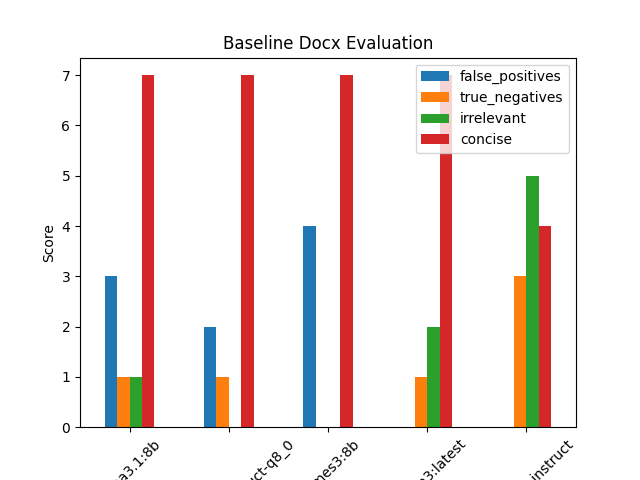
\includegraphics[width=0.8\textwidth]{baseline_docx.png}
  \caption{Evaluation outcome counts for setup A.}
  \label{fig:baseline_docx}
\end{figure}

Figure~\ref{fig:baseline_markdown} shows the distribution of evaluation outcomes
(TP, FN, IR) for setup B

\begin{figure}[H]
  \centering
  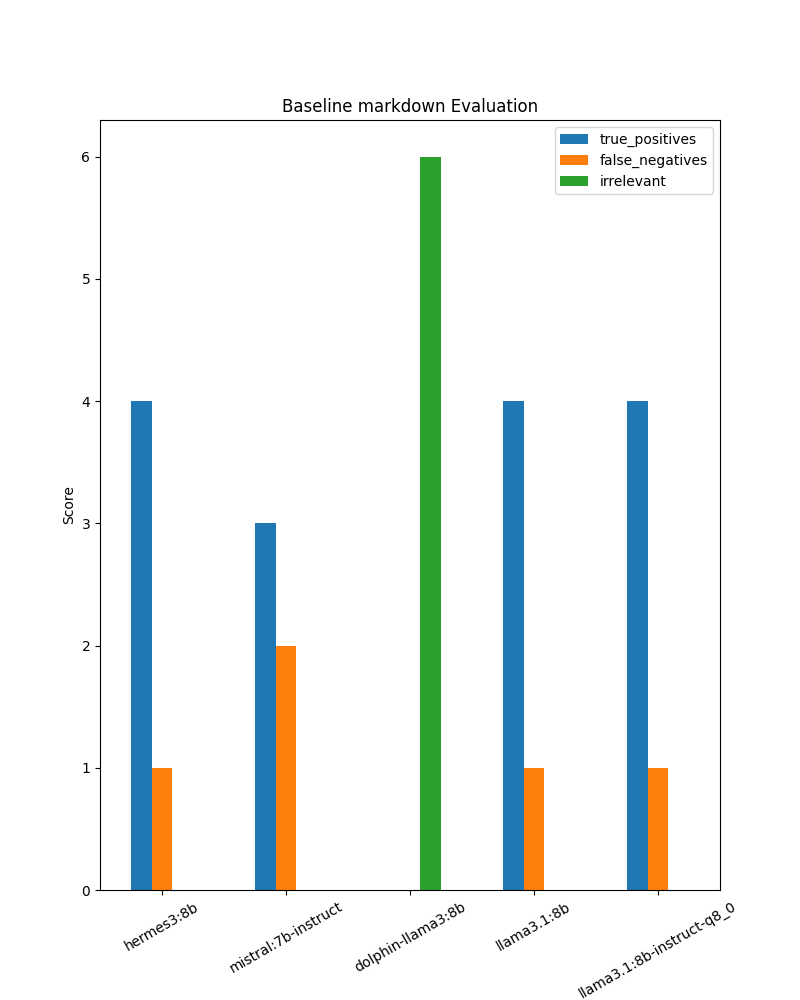
\includegraphics[width=0.8\textwidth]{baseline_markdown.png}
  \caption{Evaluation outcome counts for setup B.}
  \label{fig:baseline_markdown}
\end{figure}

Figure~\ref{fig:agentic_markdown} shows the distribution of evaluation outcomes
(TP, FN, IR) for setup C

\begin{figure}[H]
  \centering
  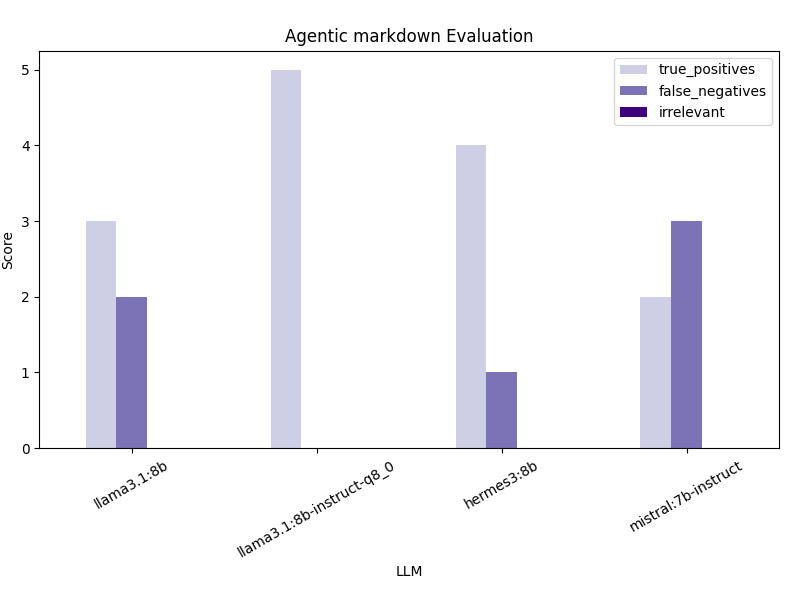
\includegraphics[width=0.8\textwidth]{agentic_markdown.png}
  \caption{Evaluation outcome counts for setup C.}
  \label{fig:agentic_markdown}
\end{figure}

Figure~\ref{fig:baseline_docxexecution_time} shows the average execution time
per document for Setup A

\begin{figure}[H]
  \centering
  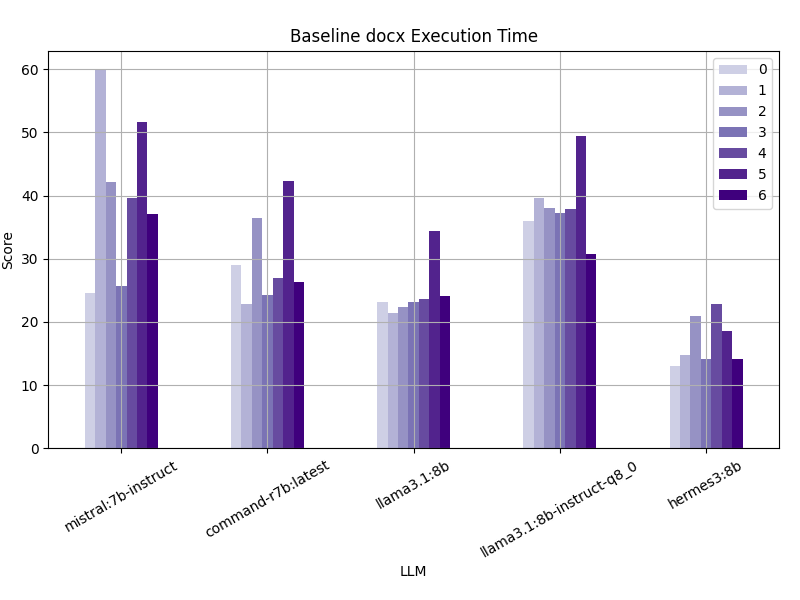
\includegraphics[width=0.8\textwidth]{baseline_docxexecution_time.png}
  \caption{Evaluation outcome counts for setup A.}
  \label{fig:baseline_docxexecution_time}
\end{figure}

Figure~\ref{fig:baseline_markdownexecution_time} shows the average execution time
per document for Setup B

\begin{figure}[H]
  \centering
  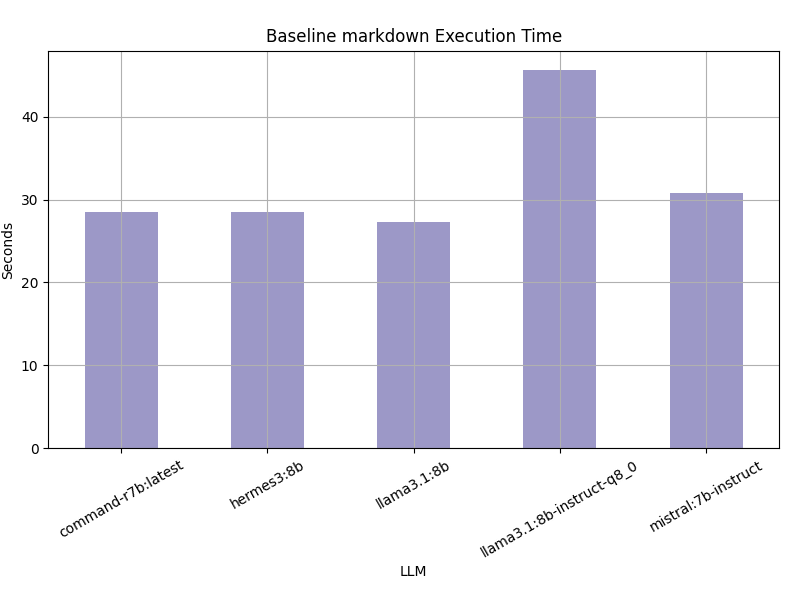
\includegraphics[width=0.8\textwidth]{baseline_markdownexecution_time.png}
  \caption{Evaluation outcome counts for setup B.}
  \label{fig:baseline_markdownexecution_time}
\end{figure}

Figure~\ref{fig:agentic_markdownexecution_time} shows the average execution
time per document for Setup C

\begin{figure}[H]
  \centering
  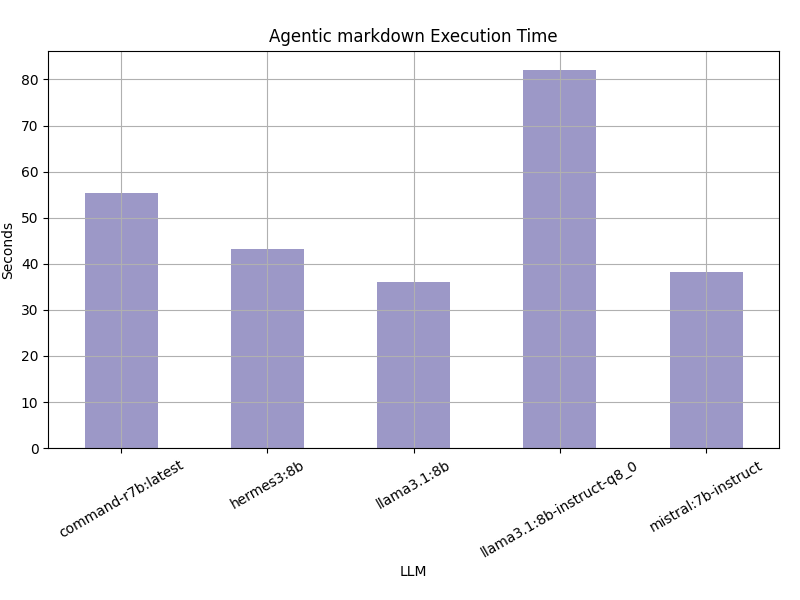
\includegraphics[width=0.8\textwidth]{agentic_markdownexecution_time.png}
  \caption{Evaluation outcome counts for setup C.}
  \label{fig:agentic_markdownexecution_time}
\end{figure}

